\documentclass[11pt]{article}
\usepackage[a4paper, margin=2cm]{geometry}
\usepackage{fancyhdr} % fancy document header
\usepackage{graphicx} % Inserting images
\usepackage[toc,page]{appendix}
\usepackage{subcaption}
\usepackage{float} % 'H' (force here) placement specifier 
\usepackage{hyperref} % Click-able citations
\usepackage{booktabs}
\usepackage{xcolor}
\usepackage{verbatim}
\usepackage{enumitem}
\usepackage[parfill]{parskip}
\usepackage[numbers,sort&compress]{natbib}
\usepackage{subscript}

\renewcommand\familydefault{\sfdefault}

% Define a command to get the word count between two sections
\newcommand{\detailtexcount}[1]{%
  \immediate\write18{texcount -merge -sum -q #1.tex output.bbl > #1.wcdetail }%
  \verbatiminput{#1.wcdetail}%
}

\fancyhead[L]{Guided Team Challenge Report}
\fancyhead[R]{\today}

\begin{document}
\pagestyle{fancy}

%TC:ignore
\begin{titlepage}
\begin{center}
\vspace*{1cm}

{\huge Automated computer vision pipeline for high-throughput phenotyping of tef shoots on top-down imagery}
    
\vspace{1.5cm}

Alexandre Shinebourne

Supervised by Dr Stéphanie Swarbreck (NIAB) and Dr Eiko Yoneki (Department of Computer Science)

\vfill

This report is submitted for the Master's project in the application of artificial intelligence for the study of environmental risks (AI4ER), which comprises part of the Master of Research qualification within the UKRI Centre for Doctoral Training.
    
\vspace{1.5cm}


\includegraphics[width=0.4\textwidth]{assets/University_of_Cambridge_logo.png}

\vspace{0.8cm}

% TODO: Date here
    
\end{center}

\newpage

\section*{Declaration}

This report is the result of my work and includes nothing which is the outcome of work done in collaboration except where expressly indicated in the text and bibliography.

\section*{Data and Code}

The code developed as part of this project is publicly available at \url{https://github.com/a-shine/niab-automated-phenotyping} \href{https://github.com/ai4er-cdt/earthquake-predictability/tree/v1.0.0}{v1.0.0}. Our data sources are available in the README at \url{https://github.com/ai4er-cdt/earthquake-predictability/blob/main/README.md#data}.

\section*{Acknowledgements}

I thank my supervisors, Stéphanie Swarbreck and Eiko Yoneki. I greatly benefited from their guidance and support.

\end{titlepage}


\begin{abstract}

\phantomsection

% TODO: Abstract
\noindent

\vspace{1cm}

\noindent\textbf{Keywords:} Automated high-throughput phenotyping, Computer Vision, Semantic segmentation, Active learning, Labelling budget

\end{abstract}

%TC:endignore
\newpage

\tableofcontents
\newpage

\section{Introduction}\label{sec:introduction}

\subsection{Context and motivation}\label{subsec:context-n-motivation}
% Phenotyping and breeding for food security and the environment
Global agriculture faces significant challenges in ensuring food security for a large population in a changing climate~\cite{furbankPhenomicsTechnologiesRelieve2011}. 
Breeders must quickly develop high-yielding crop lines that are more resilient to water strain, extreme heat, pests, and weeds.
A crop's physical characteristics and attributes are known as the phenotype and are determined by the plant's genotype~\cite{braytonPhenotyping2018}.
These characteristics determine the plant's resilience and ability to thrive.

% Shoot phenotyping for out-competing weeds in the context of tef (manually sowed, smallholder farms)
We need to develop resistant crops to sustain the food supply in East Africa, as global warming causes both waterlogging and drought. 
Tef (Eragrostis tef) is an orphan cereal crop from the region. 
The closest cultivated relative is finger millet (Eleucine coracana).
It is a type of grass well adapted to Ethiopian conditions and holds a high percentage of proteins and micronutrients (e.g., calcium, iron, and zinc).
It is an important core food~\cite{redaAchievingFoodSecurity2014, tadeleEmpiricalReviewUse2021}.

Furthermore, Tef is typically grown by smallholder farmers with limited access to machinery and crop protection.
The seeds are often sown by hand, resulting in the crops being dispersed chaotically when germinating.
This means mechanical weeding can be very challenging.
Therefore, it would be beneficial to develop breed lines that can cover the ground faster (large amounts of above-ground plant biomass).
These lines would suppress weed growth by out-competing weeds for light.

% Introduce phenotyping bottleneck problem with high throughput technique
There are several approaches to plant breeding.
A method which requires a deep understanding of the plant genotype-to-phenotype mapping, where genes are precisely edited to achieve the desired phenotypic traits.
Another approach is a high-throughput technique where a high volume of lines is created by exposing seeds to a mutation-inducing agent, increasing the probability that one of the mutated seeds will exhibit the desired phenotypic properties.
The seeds are grown, and each resulting individual is analysed to determine whether the characteristics have been achieved.
The latter approach introduces a new problem in quantitative plant science: designing automated pipelines to process the large volumes of rich data generated by the phenotyping apparatus~\cite{furbankPhenomicsTechnologiesRelieve2011, grosskinskyPlantPhenomicsNeed2015, houlePhenomicsNextChallenge2010}.
Computer vision and Deep Learning (DL) are utilised to develop semi- or fully-automated image processing pipelines.

Image-based high-throughput plant phenotyping aims to associate the characteristics of plants as observed in images to their genotype, known as phenotype-to-genotype mapping~\cite{liReviewImagingTechniques2014}. 
In order for the technique to be viable, we need to make evaluating plant characteristics as efficient and scalable as genetic screening, alleviating the data analysis bottleneck~\cite{millerComputerVisionAnalysis2007, fahlgrenLightsCameraAction2015}.

\subsection{Previous work}\label{subsec:previous-work}

% Basically a paragraph per IMPORTANT paper (eventually try and weave ideas together i.e. these guys did root phenotyping, while there did shoot phenotyping both used RGB imagery and developed initial semantic segmentation masks)

% What type of phenotyping shoot or root
% What ML models do they use + what computer vision/trad algorithm do they use to process the imagery
% What level of performance do they achieve/their conclusion

% What do they have in common? (using RGB imagery, DL for semantic segmentation, 'easy' to use for practitioners)
Previous work has been carried out on image-based, high-throughput plant phenotyping for both shoots and roots~\cite{bodnerRGBSpectralRoot2017, chaudhuryComputerVisionBased2015, chaudhuryMachineVisionSystem2019, clarkThreeDimensionalRootPhenotyping2011, daschoudhuryHolisticComponentPlant2018, fahlgrenLightsCameraAction2015, fanSegmentationGuidedDeepLearning2022, guoIlluminationInvariantSegmentation2013, guoEasyPCCBenchmarkDatasets2017, henkeSemiAutomatedGroundTruth2021, hutherARADEEPOPSISAutomatedWorkflow2020, leeAutomatedHighthroughputPlant2018, liReviewImagingTechniques2014, luoEff3DPSeg3DOrganLevel2023, muhlichMeasuringPlantRoot2008, narisettiDeepLearningBased2022, smithSegmentationRootsSoil2020, yatesNewImagingMachinelearning2021}.
While some works focus on root phenotyping~\cite{bodnerRGBSpectralRoot2017, clarkThreeDimensionalRootPhenotyping2011, muhlichMeasuringPlantRoot2008, smithSegmentationRootsSoil2020}, others develop tools and methods for shoot phenotyping~\cite{chaudhuryComputerVisionBased2015, chaudhuryMachineVisionSystem2019, daschoudhuryHolisticComponentPlant2018, fanSegmentationGuidedDeepLearning2022, guoIlluminationInvariantSegmentation2013, guoEasyPCCBenchmarkDatasets2017, henkeSemiAutomatedGroundTruth2021, hutherARADEEPOPSISAutomatedWorkflow2020, leeAutomatedHighthroughputPlant2018, luoEff3DPSeg3DOrganLevel2023, narisettiDeepLearningBased2022}.
Many of the pipelines developed use a single (or time-series collection) of RGB (Red, Green and Blue) imagery, although some look at other hyperspectral imagery, notably for studying roots as they are more visible under UV light~\cite{bodnerRGBSpectralRoot2017, wassonPortableFluorescenceSpectroscopy2016}.
Some experimental setups use camera arrays or robotic manipulation of a single camera to capture several angles and observe characteristics that can only be measured in three dimensions~\cite{chaudhuryComputerVisionBased2015, chaudhuryMachineVisionSystem2019, clarkThreeDimensionalRootPhenotyping2011}.

A common step across the image processing pipelines is semantic segmentation of the shoot or root from imagery.
This allows for further processing to determine phenotypic characteristics such as root length, root width, root or shoot branching factor, leaf count and shoot area.
Segmentation tends to be semantic, so the image is divided into several segments for detected objects, but there is no distinction between different instances of the same object.
Traditional computer vision segmentation techniques include HSV (Hue Saturation Value) thresholds, which classify whether or not pixels belong to an object by determining bounds for Hue Saturation values~\cite{adamsPlantSegmentationSupervised2020}.
However, more recent papers opt for a DL approach over traditional non-ML approaches due to the optical variability in plant appearances~\cite{narisettiDeepLearningBased2022}.
For shoot segmentation, the U-Net architecture~\cite{ronnebergerUNetConvolutionalNetworks2015} is commonly used due to its simple implementation and effectiveness~\cite{narisettiDeepLearningBased2022, whiteGeneratingSegmentationMasks2020}.
In addition, several off-the-shelf models for root and shoot segmentation, such as DeepShoot~\cite{narisettiDeepLearningBased2022} and Root Painter~\cite{smithOotAinterDeep2022} are available, so others can more easily build segmentation into their pipelines.

% (i.e. these papers all do shoot phenotyping, one looking at multiple individuals, in greenhouse, in fields...)
Of the papers focused on shoot phenotyping, several have developed image processing pipelines for top-down imagery~\cite{fanSegmentationGuidedDeepLearning2022, guoIlluminationInvariantSegmentation2013, ronnebergerUNetConvolutionalNetworks2015, hutherARADEEPOPSISAutomatedWorkflow2020, leeAutomatedHighthroughputPlant2018, narisettiDeepLearningBased2022} and side-on imagery~\cite{daschoudhuryHolisticComponentPlant2018, narisettiDeepLearningBased2022}. 
For use in high-throughput phenotyping, the data inferred from an image must be associated with an individual genotype, so images usually contain a single individual.
However, \textit{Lee et al.}~\cite{leeAutomatedHighthroughputPlant2018} have developed a phenotyping platform with several trays of individuals and a camera on two motor-controlled axes.
The camera moves from tray to tray to take regular images from above throughout the plant growth cycle.
While most phenotyping platforms are setup in labs or greenhouses in order to better control lighting and protect apparatus such as cameras for capturing images, \textit{Guo et al.}~\cite{guoIlluminationInvariantSegmentation2013, guoEasyPCCBenchmarkDatasets2017} capture image data on phenotyping platform in open field environments.
This has the advantage of measuring crop properties in a more natural environment, where crops are exposed to natural conditions and soil.
In addition, crops seldom grow in isolated environments, and their development can be impacted by interaction with neighbouring individuals~\cite{finchWheatRootLength2017}, so monitoring the individual genotype behaviours in a multi-crop environment is important.
A notable limitation of taking imagery in open field conditions is wind can move the shoots and leaves, causing segmentation to fail and making identification of individuals very difficult, which limits its use case for phenotype-to-genotype mapping~\cite{guoEasyPCCBenchmarkDatasets2017}.

The development of image-based, high-throughput plant phenotyping pipelines is an interdisciplinary effort between plant science and engineering for designing the phenotyping platform, as well as computer science for image processing involving computer vision and ML.
In previous work, while the developed processing technique is coupled to particular phenotyping and imaging platforms, some have attempted to make parts of the pipeline available for use by others~\cite{hutherARADEEPOPSISAutomatedWorkflow2020, henkeSemiAutomatedGroundTruth2021, guoEasyPCCBenchmarkDatasets2017, narisettiDeepLearningBased2022}.
Moving forward, a clear priority is developing tooling that can be re-used between different platforms and by plant scientists without the need for a Computer vision or ML background.
\textit{Narisetti et al.}~\cite{narisettiDeepLearningBased2022}, and \textit{Smith et al.}~\cite{smithSegmentationRootsSoil2020}, put forward a Graphical User Interface (GUI) software that allows practitioners to segment out the shoots or roots respectively for several common crop varieties.

% Introduce the notion of logic-based (graphs) for post-processing images once segmented and plotting temporal evolution of crop development
In \textit{Muhlich et al.}'s~\cite{muhlichMeasuringPlantRoot2008} on measuring plant root growth and development, the plants are grown in a transparent growth medium, allowing for easy, non-invasive imagery of the plant root system.
The team uses nonlinear filters to isolate the roots and then a graph-based approach to follow each of the roots.
There is the notable problem of distinguishing between when root branches into sub-roots or two independent roots crossing.
They use traditional logic-based techniques to classify root crossings and branches.
Once they are able to identify each of the primary roots and branches, they integrate temporal information and plot the growth of the complete root system as well as the contribution of different root orders over time.
Like \textit{Muhlich et al.}'s~\cite{muhlichMeasuringPlantRoot2008}, \textit{Choudhury et al.}~\cite{daschoudhuryHolisticComponentPlant2018} use 2D imagery, temporal image sequences and a graph-based approach to monitor crop development, in their case maize plants, focusing on the above ground numbers of leaves and the individual leaf growth.
In addition to developing novel computer vision algorithms for automated detection of individual leaves and the stem they have also made a publicly available benchmark dataset of side on plant images.

% Discuss PCCr and other phenotypic metrics determined from image pipelines
\textit{Gui et al.}~\cite{guoEasyPCCBenchmarkDatasets2017} developed a tool for high throughput measurements of the plant canopy coverage ratio under field conditions.
They choose to develop an image proceeding pipeline that measures the plant canopy coverage ratio (PCCr) as it is a good indicator of plant growth status and correlates with the leaf area index, canopy light interception, nitrogen content, and crop yield~\cite{campilloUsingDigitalImages2008, casadesusUsingVegetationIndices2007}.
In addition, it is a good metric to measure from top-down imagery as it is defined as "the percentage of the orthogonal projection area relative to the area of crop foliage in the horizontal plane"~\cite{guoEasyPCCBenchmarkDatasets2017}.

% Main limitation of previous techniques (not adaptable, often not phenotyping with neighbouring plants - plants interacting between each other (\cite{finchWheatRootLength2017}))
An overarching limitation of the previous work is that the image processing pipeline is tightly coupled to the experimental procedure/design, limiting the generalizability of the technique despite general parts of the pipelines being generally applicable, such as the root segmentation model.
When using non-ML segmentation different experimental setups and camera placements represent a major obstacle in the efficient and accurate processing and analysis of large volumes of image data~\cite{minerviniImageAnalysisNew2015}.
In addition, many of the phenotyping platforms, particuallty setup on lab environments only have one crop per pot.
While this makes image analysis easier it would be beneficial to observe plants growing in communities~\cite{finchWheatRootLength2017} while still being able to map an individual to it's genotype.

\subsection{Research aims}\label{subsec:research-aims} % Overarching aim and specific research questions

Being able to track single plants growing alongside neighbours is paramount to the selection of new crop varieties that are resilient against weeds and well adapted to co-cultivating conditions. The project addresses developing an image-analysis-based method that would allow assessment of the development of the canopy over time, using images acquired in testing a plant's 45 mutant population. In this project, we focus on working the Tef, a popular crop in Ethiopia.

We will track the development of young shoots as they germinate to determine which shoots develop fastest and, hence, can outcompete weeds during the most vulnerable period of the crop's lifecycle for weed-related issues.

In the process, we will evaluate the feasibility of image-based, high-throughput plant phenotyping of shoots from top-down imagery on the NIAB dataset. We will explore, unlike previous work, how an image-based processing pipeline can be retrofitted to an existing dataset rather than designing a phenotyping platform specifically with an image-processing pipeline in mind.

As part of the project, we will develop a robust semantic segmentation ML model for young Tef shoots. We will determine which model architectures perform best, how annotation quality affects model performance, and how to deal with low annotation budgets with an active learning approach. Like previous work~\cite{smithOotAinterDeep2022, narisettiDeepLearningBased2022}, we will make the model available publicly for use in further research.

% Make a numbered list of research questions that I can refer too

\clearpage
\section{Data and methods}\label{sec:data-n-methods}

\subsection{Data}\label{subsec:data}

% Explain the apparatus and experimental technique

% Ran 5 experiments
% The blocks all my replicates in one side of the glasshouse
% Within the blocks they are all genetically different and in each block they have the same combinations
% 16 plants per plot
% Mutant population 

% 16 genotypes * 40 plots = 1 block each plant is genetically unique
% We need to link a specific genotype to a biomass
% Dsicovery system for genotypes - you create many random mutations and see if they exhibit this behaviour but because it is a random it needs to be done with manny genotypes

% This explains why the seeds are planted in transparent pots with the each seed planted just by the pot rim
Similarly,  \textit{Smith et al.}~\cite{smithSegmentationRootsSoil2020}have developed a pre-trained model for root segmentation from the side on transparent pot imagery. This technique has been developed for root segmentation where the seed is either planted in a transparent medium or planted in compost at the pot rim so shoots can be observed non-invasively.

% Explain manually annotating 280 images for training segmentation model using a semi-automated annotation pipeline

\subsection{Methods}\label{subsec:methods}

\begin{figure}
    \centering
    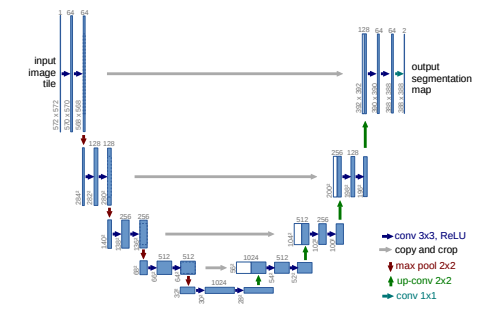
\includegraphics[width=0.5\linewidth]{assets//01_introduction/Screenshot 2024-05-22 at 16.06.04.png}
    \caption{Enter Caption}
    \label{fig:enter-label}
\end{figure}

U-Net was initially conceived for segmentation tasks in medical imaging but has seen widespread adoption in DL and Computer vision.
% TODO: basic background on U-Net with reference diagram (this should probably be moved to the methods section)
The U-Net model consists of two parts, which are mirror images of each other (see Figure~\ref{}).
The initial encoder part of the model takes the input image (or a smaller tile from the input image) and repeatedly applies convolution, followed by ReLU activation and Max pooling operations.
This reduces the spatial dimension of the image, producing a deep feature map.
This representation is then passed to the decoder part of the model with convolution layers that gradually increase the spatial dimension of the image, back to its original size.
U-Net also includes jump connections that connects the

\clearpage
\section{Results and discussion}\label{sec:results-n-dicussion}


\clearpage
\section{Conclusion}\label{sec:conclusion}

%TC:ignore
\clearpage
\bibliographystyle{vancouver}
\bibliography{bibliography}

\clearpage
\appendix

\section{Glossary}

\noindent
\begin{tabular}{lp{9cm}}
\toprule
\textbf{Term} & \textbf{Definition} \\
\midrule
\bottomrule
\end{tabular}

\clearpage

% \detailtexcount{main}

%TC:endignore

\end{document}
